\documentclass{article}
\usepackage{parskip}
\usepackage{pdfpages}
\usepackage{hyperref}
\usepackage{amsmath}
\usepackage[margin=.6in]{geometry}
\begin{document}
missed lecture due to vacation
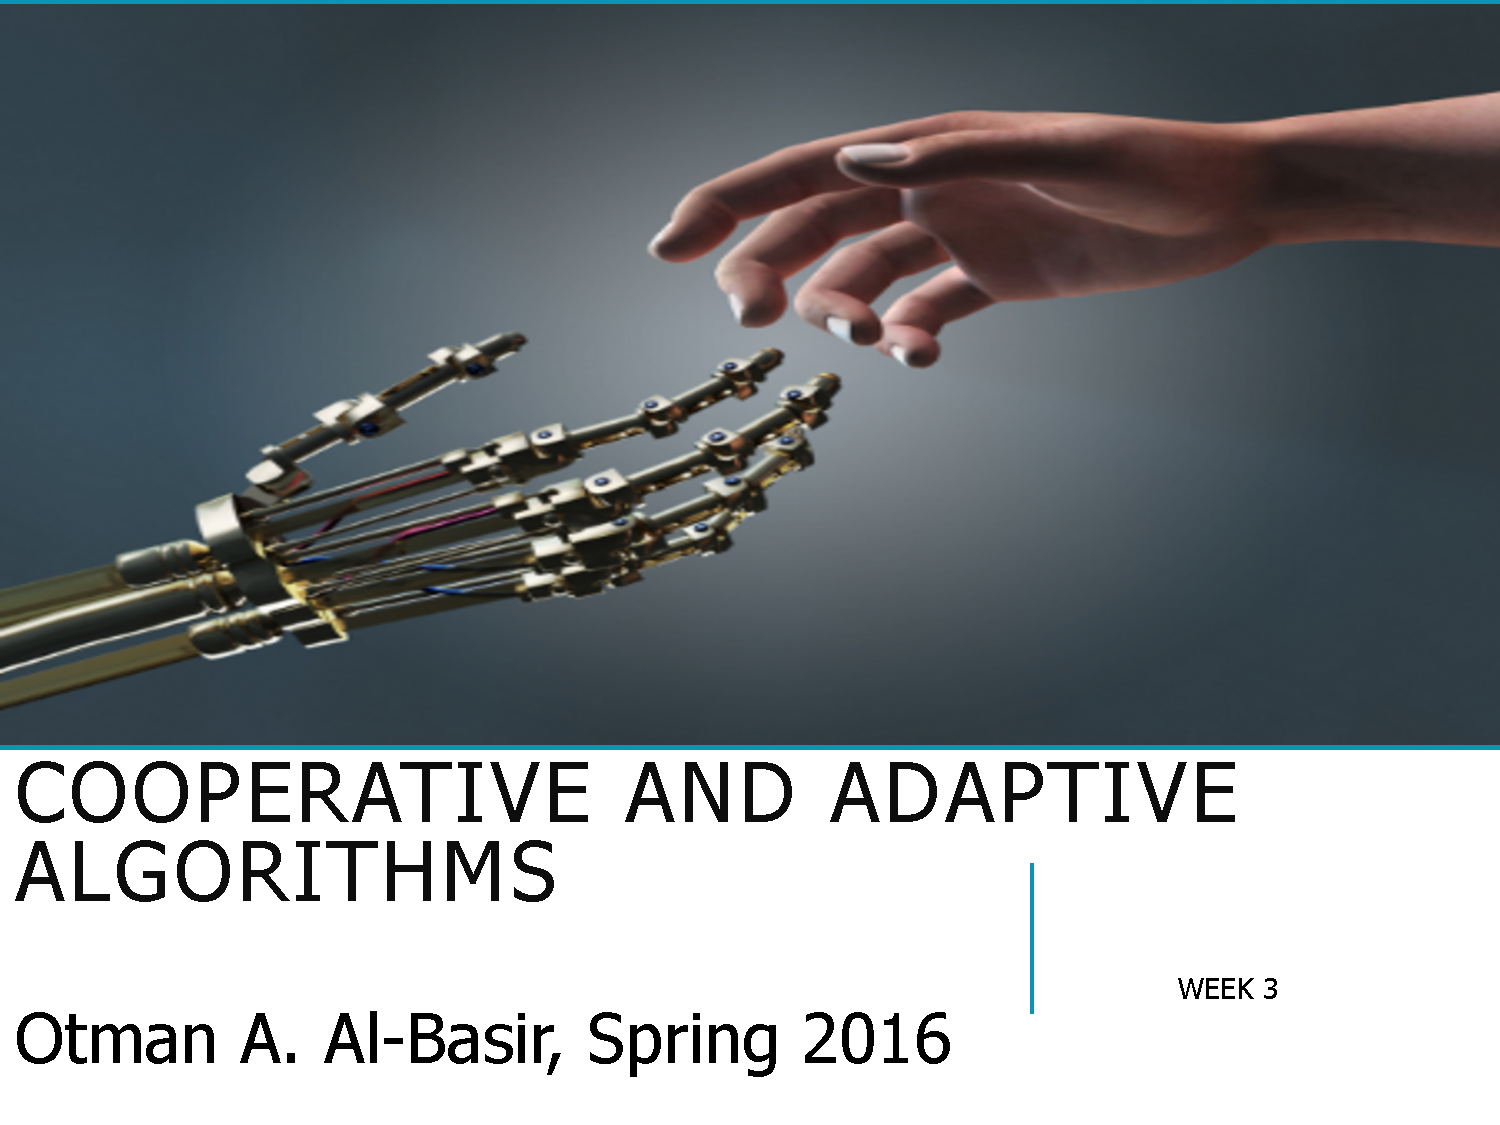
\includepdf[pages=1-32]{slides}
IF the classes cannot be separated by a line or hyperplane, then we cannot use the perceptron, a different approach is required.

\includepdf[pages=33]{slides}
We need to update our weights and bias only if they change between the labeled output and actual output is too far apart. This is denoted with $\delta\omega_i$. Each cycle of adjusting weights is one epoch.

The training signal is the signal used to shape the pattern. We give it a certain location and angle with respect to the space. The system learns from this and adjusts itself so that it matches the learned data. If we have not achieved this after one epoch we start over. The system starts to shave its boundary to become more accurate.

This is a classifier system, trying to find the boundary between classes.

\includepdf[pages=34-37]{slides}
Once we teach the system properly we need to generalize it to be able to handle unlabeled data. Perceptrons are not create at generalization. Good at classification.

We start with an initial random boundary. It really doesn't work as seen by the graph (red line).

\includepdf[pages=37]{slides}
The perceptron has many issues. It cannot deal with non linearly seperable data. Another problem is that its line to separate the classes is not optimal which makes it a terrible generalizer (this is a good example of a question that might be on the exam).

\includepdf[pages=38]{slides}
We are now looking at the Adaline system so that we can optimize the line drawn.

Say we have a weight vectory $\omega$ and a set of data $x$. We multiply these two vectors to get a scalar and apply a function to it to get the output of the system, $o$. The function $f$ could be a step function or a signal function. For now we assume that it is a step function. We provide some labeled values $t$. The error between $t$ and $o$ is called $E$ and we want to decrease this to 0 as we train the system. This decaying is the gradient of the function (or the derivative) for multivariable function.

$E = (o-t)^2$ We square this because we want the error to be positive.

We dont want $o$ to be the outcome of the system in the perceptron. We don't want to use the gradient in the perceptron because the possible outputs are +1 or -1 because we are dealing with a signal function. We have to take the derivative but the perceptron gives discrete numbers which we cannot work with. We take the output of the perceptron $o_{artificial}$ and pass it through the signal function to get the actual output $o$. So when we get the error its relative to the artificial o.

Now we can take the derivative relative to $\omega$

\[
	\nabla_\omega = 2(o_a - t)\frac{\delta\omega x}{\delta\omega}
	=  2(o_a - t)x
\]
we try to minimize this which will give us the optimal line.

\includepdf[pages=39-43]{slides}
The adeline is much better at handling noisy data.

\includepdf[pages=44]{slides}
The Adeline still cannot handle nonlinear data. It has the same issue as the perceptron.

Some people tried to get around this by attaching some adeline together. This was very costly. It only works for veeeeeeery simple cases.

\includepdf[pages=45]{slides}
Sometimes you have a problem that is not linearly separable with a single line, but you can separate them with lines that you and together. We also might want to try to find clusters, this cannot be done with the perceptron or the adeline. The solution to this is multi-layer perceptron (MLP).

\includepdf[pages=46-61]{slides}














\end{document}

